\clearpage
\thispagestyle{empty}
~\clearpage
%\graphicspath{{Figures_chapter-3/}}
%\chapter{A class of finite difference schemes for circular interface problems with an HOC approach}
\chapter{Case Study I}
\label{chap3}
\section{Experiment Design}
In our study, we demonstrated the ability of HackIT tool as a single-player platform for conducting experiments.The timing of deception was manipulated across two conditions: early deception (N = 8) and late deception (N = 8). The total number of servers were 40, where 20 web-servers were assigned as honeypot web-servers during deception rounds. In both conditions, participants playing as hackers were given 6 game rounds in a sequence (end point unknown to participants), where 2 game rounds possessed deception. 
\FloatBarrier
\begin{figure}[!htbp]
\centering
  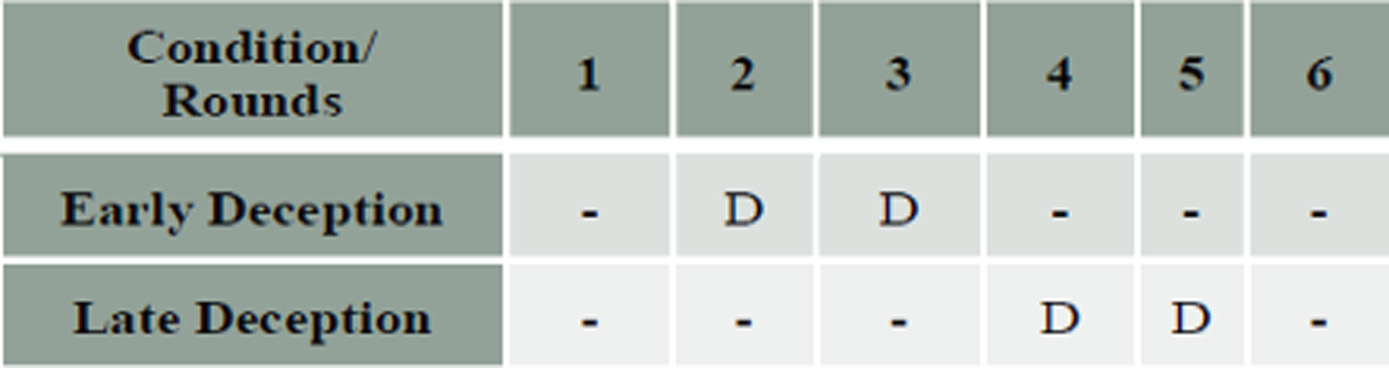
\includegraphics[scale=0.2]{Chap3/rounds.png}
  \caption{Experiment design using deception game\\D: Deception present -: Deception not present}\label{fig:figure8}
\end{figure}

In this experiment, if the timing of deception was early, then deception was present on the second and third rounds in the sequence. However, if the timing of deception was late, then deception was present in the fourth and fifth rounds in the sequence as shown in Figure \ref{fig:figure8}. The honeypots were easy to exploit via common ports and vulnerabilities in the deception rounds compared to the non-deception rounds, where there were no honeypots. However, participants were not told that honeypots will involve easy to attack configurations in deception rounds. Also, participants were not disclosed the rounds on which deception was involved. To analyze human data, we looked at the proportion of honeypot attacks and proportion of regular attacks at the attack stage by the hacker across six-rounds in each condition. These proportions were calculated by average the attack decision over all the trials and participants. We also calculated frequency of each exploits used on regular and honeypots in deception and no-deception trials.

\section{HackIT Task}
The objective of attacker in HackIT was to steal real credit-card information located on one of the webservers.We first configured the network with 40 webservers where 20 webservers acted as honeypots. We also set up a strategy where honeypots were easier to attack during the deception rounds. Based on these strategies, in this experiment, we used different configurations shown in \ref{fig:figure7}. For example, a system with Windows XP operating system, port 80/tcp, and service http was easily exploitable. Such a configuration was mapped to a honeypot. However, a system with Linux operating system, port 22/tcp and service ssh was difficult to
attack. Such a configuration was mapped to a regular webserver. Participants were informed about the easy to exploit and the difficult to exploit configurations in \ref{fig:figure7} as part of the instructions.

\FloatBarrier
\begin{figure}[!htbp]
\centering
  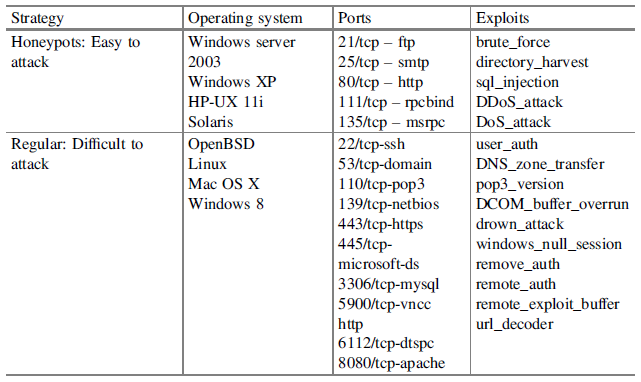
\includegraphics[scale=0.6]{Chap3/exploits.PNG}
  \caption{Configuration of honeypot and regular system}\label{fig:figure7}
\end{figure} 
First, the attacker probed the network using nmap command to gain information about different web-servers. Probing different web-servers gave the information about the operating system, open ports, services, and vulnerabilities. The information provided to the attacker as a result of probing systems gave him an idea about the type of configuration on the probed system. Once the attacker collects information about open ports and services, he could attack a web-server by using the \enquote{use\_exploit} command.
The use\_exploit command exploited vulnerabilities on a system and helped the attacker to gain access to that web-server. Next, the attacker could list different files on the exploited web-server by using the “ls” command. Next, the attacker could transfer required files containing credit card information (e.g., \enquote{pin.txt}) using the \enquote{scp} command. After attackers copied the file from the exploited system, he was informed whether he was successful or not in stealing a real credit-card file from the computer via a text-based feedback.
\section{Participants}
Participation was voluntary and a total of 16 male participants participated in the study that was advertised via an email advertisement. Out of the 16 people, 62.5\% people had taken a course in computer networks/security. The age of participants ranged from 18\textendash 22 years. About 56\% were 3rd year and 44\% were final year undergraduate students from Indian Institute of Technology Mandi, India. All the participants were remunerated at a fixed rate of INR 50 for their participation in the study.

\section{Procedure}
Participants were given instructions about their objective in the HackIT task, and they were informed about their own action’s payoffs. Specifically, human hackers were asked to maximize their payoff by stealing the real credit-card file from the network over several rounds of play (participants were not aware of the endpoint of the game).Each round had two stages: Probe stage and Attack stage. Hacker could probe the network using \enquote{nmap} utility in first stage. After probing the web-servers, he received information about open ports, operating systems, services, and vulnerabilities associated with different web-server. Next, the hacker had to choose one web-server to exploit and exploit web-servers using “use\_exploit” command during attack stage. Once the web-server was exploited, hackers transferred the credit-card file to their remote computer.

\section{Results and Analysis}
Figure \ref{fig:figure9} shows the proportion of attacks on honeypot and regular web-servers. There was no difference in the proportion of attacks in late and early deception conditions.
\FloatBarrier
\begin{figure}[!htbp]
\centering
  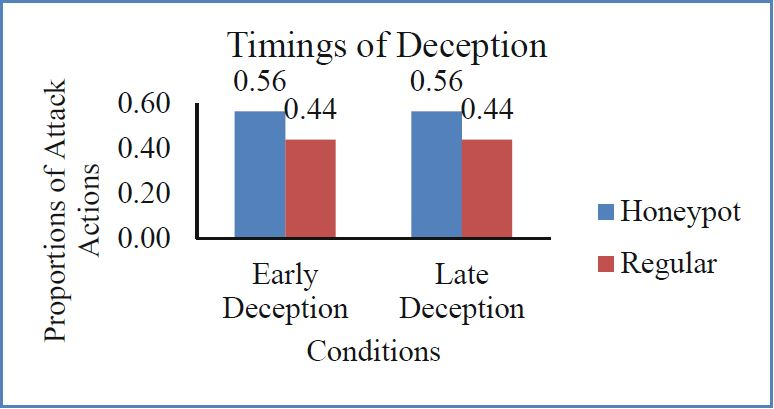
\includegraphics[scale=0.6]{Chap3/study1_graph.jpg}
  \caption{Proportion of attack actions on regular and honeypot webservers across rounds and participants}\label{fig:figure9}
\end{figure} 
Next, we analyzed the exploits used during deception rounds and non-deception rounds by participants. When regular (honeypot) systems are attacked during deception rounds, that is called as deception failure (success). Figure \ref{fig:figure10} and \ref{fig:figure11} show the number of regular attacks and honeypot attacks against different exploits in deception failure and success, respectively. During deception failure, the remote\_auth vulnerability was more exploited in early condition compared to late condition and the pop3\_version vulnerability was exploited more in the late condition compared to early condition.  During deception success, the brute\_force vulnerability was more exploited more in early condition compared to late condition and the DOS\_attack and sql\_injection vulnerabilities were exploited more in the late condition compared to early condition.
\FloatBarrier
\begin{figure}[!htbp]
\centering
  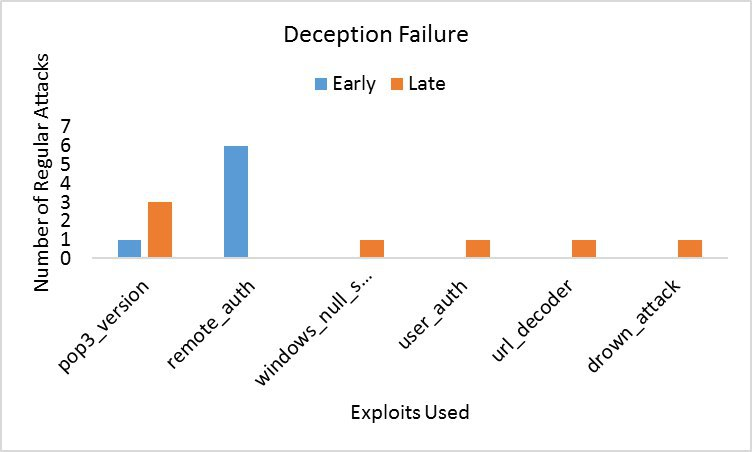
\includegraphics[scale=0.6]{Chap3/failure.jpg}
  \caption{Vulnerability exploited on regular systems in deception rounds}\label{fig:figure11}
\end{figure} 
\FloatBarrier
\begin{figure}[!htbp]
\centering
  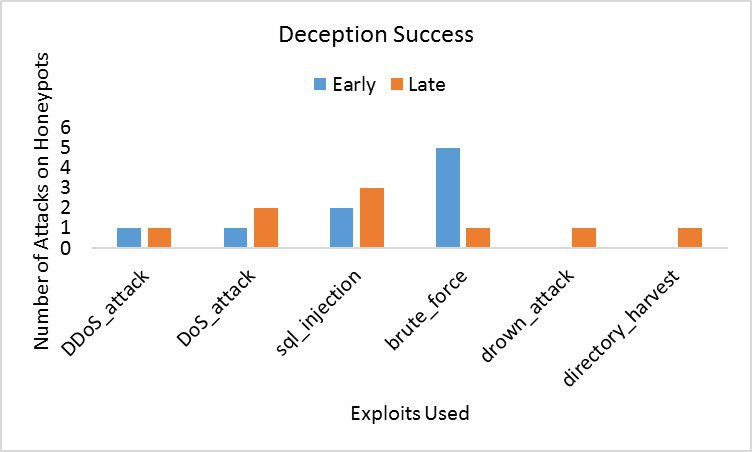
\includegraphics[scale=0.6]{Chap3/success.jpg}
  \caption{Vulnerability exploited on honeypots in deception rounds}\label{fig:figure10}
\end{figure} 
Figure \ref{fig:figure12} shows the number of attacks on regular web-servers using different vulnerabilities. We found that during early deception conditions, mostly hackers used remote\_auth and drown\_attack vulnerabilities. Furthermore, during late deception condition, hackers used pop3\_version and remote\_auth vulnerabilities.
\FloatBarrier
\begin{figure}[!htbp]
\centering
  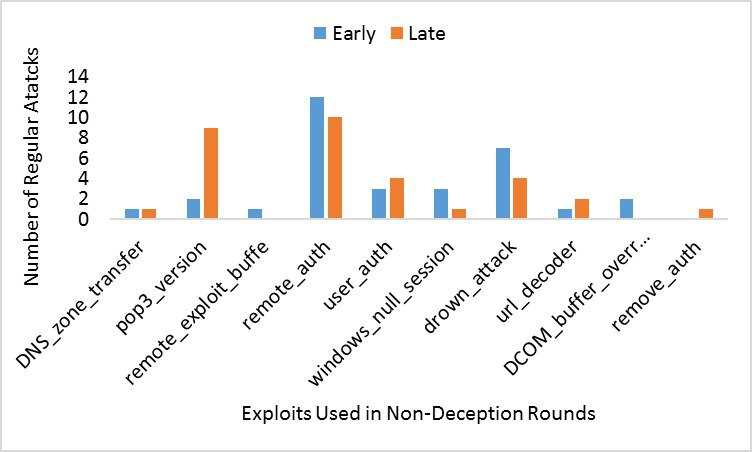
\includegraphics[scale=0.6]{Chap3/non-deception.jpg}
  \caption{Vulnerability exploited in non-deception rounds}\label{fig:figure12}
\end{figure} 
\clearpage 
